\documentclass[]{tufte-handout}

% ams
\usepackage{amssymb,amsmath}

\usepackage{ifxetex,ifluatex}
\usepackage{fixltx2e} % provides \textsubscript
\ifnum 0\ifxetex 1\fi\ifluatex 1\fi=0 % if pdftex
  \usepackage[T1]{fontenc}
  \usepackage[utf8]{inputenc}
\else % if luatex or xelatex
  \makeatletter
  \@ifpackageloaded{fontspec}{}{\usepackage{fontspec}}
  \makeatother
  \defaultfontfeatures{Ligatures=TeX,Scale=MatchLowercase}
  \makeatletter
  \@ifpackageloaded{soul}{
     \renewcommand\allcapsspacing[1]{{\addfontfeature{LetterSpace=15}#1}}
     \renewcommand\smallcapsspacing[1]{{\addfontfeature{LetterSpace=10}#1}}
   }{}
  \makeatother

\fi

% graphix
\usepackage{graphicx}
\setkeys{Gin}{width=\linewidth,totalheight=\textheight,keepaspectratio}

% booktabs
\usepackage{booktabs}

% url
\usepackage{url}

% hyperref
\usepackage{hyperref}

% units.
\usepackage{units}


\setcounter{secnumdepth}{-1}

% citations
\usepackage{natbib}
\bibliographystyle{plainnat}


% pandoc syntax highlighting
\usepackage{color}
\usepackage{fancyvrb}
\newcommand{\VerbBar}{|}
\newcommand{\VERB}{\Verb[commandchars=\\\{\}]}
\DefineVerbatimEnvironment{Highlighting}{Verbatim}{commandchars=\\\{\}}
% Add ',fontsize=\small' for more characters per line
\newenvironment{Shaded}{}{}
\newcommand{\AlertTok}[1]{\textcolor[rgb]{1.00,0.00,0.00}{\textbf{#1}}}
\newcommand{\AnnotationTok}[1]{\textcolor[rgb]{0.38,0.63,0.69}{\textbf{\textit{#1}}}}
\newcommand{\AttributeTok}[1]{\textcolor[rgb]{0.49,0.56,0.16}{#1}}
\newcommand{\BaseNTok}[1]{\textcolor[rgb]{0.25,0.63,0.44}{#1}}
\newcommand{\BuiltInTok}[1]{\textcolor[rgb]{0.00,0.50,0.00}{#1}}
\newcommand{\CharTok}[1]{\textcolor[rgb]{0.25,0.44,0.63}{#1}}
\newcommand{\CommentTok}[1]{\textcolor[rgb]{0.38,0.63,0.69}{\textit{#1}}}
\newcommand{\CommentVarTok}[1]{\textcolor[rgb]{0.38,0.63,0.69}{\textbf{\textit{#1}}}}
\newcommand{\ConstantTok}[1]{\textcolor[rgb]{0.53,0.00,0.00}{#1}}
\newcommand{\ControlFlowTok}[1]{\textcolor[rgb]{0.00,0.44,0.13}{\textbf{#1}}}
\newcommand{\DataTypeTok}[1]{\textcolor[rgb]{0.56,0.13,0.00}{#1}}
\newcommand{\DecValTok}[1]{\textcolor[rgb]{0.25,0.63,0.44}{#1}}
\newcommand{\DocumentationTok}[1]{\textcolor[rgb]{0.73,0.13,0.13}{\textit{#1}}}
\newcommand{\ErrorTok}[1]{\textcolor[rgb]{1.00,0.00,0.00}{\textbf{#1}}}
\newcommand{\ExtensionTok}[1]{#1}
\newcommand{\FloatTok}[1]{\textcolor[rgb]{0.25,0.63,0.44}{#1}}
\newcommand{\FunctionTok}[1]{\textcolor[rgb]{0.02,0.16,0.49}{#1}}
\newcommand{\ImportTok}[1]{\textcolor[rgb]{0.00,0.50,0.00}{\textbf{#1}}}
\newcommand{\InformationTok}[1]{\textcolor[rgb]{0.38,0.63,0.69}{\textbf{\textit{#1}}}}
\newcommand{\KeywordTok}[1]{\textcolor[rgb]{0.00,0.44,0.13}{\textbf{#1}}}
\newcommand{\NormalTok}[1]{#1}
\newcommand{\OperatorTok}[1]{\textcolor[rgb]{0.40,0.40,0.40}{#1}}
\newcommand{\OtherTok}[1]{\textcolor[rgb]{0.00,0.44,0.13}{#1}}
\newcommand{\PreprocessorTok}[1]{\textcolor[rgb]{0.74,0.48,0.00}{#1}}
\newcommand{\RegionMarkerTok}[1]{#1}
\newcommand{\SpecialCharTok}[1]{\textcolor[rgb]{0.25,0.44,0.63}{#1}}
\newcommand{\SpecialStringTok}[1]{\textcolor[rgb]{0.73,0.40,0.53}{#1}}
\newcommand{\StringTok}[1]{\textcolor[rgb]{0.25,0.44,0.63}{#1}}
\newcommand{\VariableTok}[1]{\textcolor[rgb]{0.10,0.09,0.49}{#1}}
\newcommand{\VerbatimStringTok}[1]{\textcolor[rgb]{0.25,0.44,0.63}{#1}}
\newcommand{\WarningTok}[1]{\textcolor[rgb]{0.38,0.63,0.69}{\textbf{\textit{#1}}}}

% table with pandoc
\usepackage{longtable,booktabs,array}
\usepackage{calc} % for calculating minipage widths
% Correct order of tables after \paragraph or \subparagraph
\usepackage{etoolbox}
\makeatletter
\patchcmd\longtable{\par}{\if@noskipsec\mbox{}\fi\par}{}{}
\makeatother
% Allow footnotes in longtable head/foot
\IfFileExists{footnotehyper.sty}{\usepackage{footnotehyper}}{\usepackage{footnote}}
\makesavenoteenv{longtable}

% multiplecol
\usepackage{multicol}

% strikeout
\usepackage[normalem]{ulem}

% morefloats
\usepackage{morefloats}


% tightlist macro required by pandoc >= 1.14
\providecommand{\tightlist}{%
  \setlength{\itemsep}{0pt}\setlength{\parskip}{0pt}}

% title / author / date
\title[Shifting Baselines Handout]{Shifiting Baselines}
\author{Marc Los Huertos}
\date{2023-11-28}


\begin{document}

\maketitle




\hypertarget{what-are-shifting-baselines}{%
\section{What are Shifting
Baselines?}\label{what-are-shifting-baselines}}

\hypertarget{headings}{%
\section{Headings}\label{headings}}

\newthought{In his later books}\footnote{\href{https://www.edwardtufte.com/tufte/books_be}{Beautiful
  Evidence}}, Tufte starts each section with a bit of vertical space, a
non-indented paragraph, and sets the first few words of the sentence in
small caps. To accomplish this using this style, call the
\texttt{newthought()} function in \textbf{tufte} in an \emph{inline R
expression} \texttt{\textasciigrave{}r\ \textasciigrave{}} as
demonstrated at the beginning of this paragraph.\footnote{Note you
  should not assume \textbf{tufte} has been attached to your R session.
  You should either \texttt{library(tufte)} in your R Markdown document
  before you call \texttt{newthought()}, or use
  \texttt{tufte::newthought()}.}

\hypertarget{figures}{%
\section{Figures}\label{figures}}

\hypertarget{margin-figures}{%
\subsection{Margin Figures}\label{margin-figures}}

Images and graphics play an integral role in Tufte's work. To place
figures in the margin you can use the \textbf{knitr} chunk option
\texttt{fig.margin\ =\ TRUE}. For example:

\begin{Shaded}
\begin{Highlighting}[]
\FunctionTok{library}\NormalTok{(ggplot2)}
\NormalTok{mtcars2 }\OtherTok{\textless{}{-}}\NormalTok{ mtcars}
\NormalTok{mtcars2}\SpecialCharTok{$}\NormalTok{am }\OtherTok{\textless{}{-}} \FunctionTok{factor}\NormalTok{(}
\NormalTok{  mtcars}\SpecialCharTok{$}\NormalTok{am, }\AttributeTok{labels =} \FunctionTok{c}\NormalTok{(}\StringTok{\textquotesingle{}automatic\textquotesingle{}}\NormalTok{, }\StringTok{\textquotesingle{}manual\textquotesingle{}}\NormalTok{)}
\NormalTok{)}
\FunctionTok{ggplot}\NormalTok{(mtcars2, }\FunctionTok{aes}\NormalTok{(hp, mpg, }\AttributeTok{color =}\NormalTok{ am)) }\SpecialCharTok{+}
  \FunctionTok{geom\_point}\NormalTok{() }\SpecialCharTok{+} \FunctionTok{geom\_smooth}\NormalTok{() }\SpecialCharTok{+}
  \FunctionTok{theme}\NormalTok{(}\AttributeTok{legend.position =} \StringTok{\textquotesingle{}bottom\textquotesingle{}}\NormalTok{)}
\end{Highlighting}
\end{Shaded}

\begin{marginfigure}
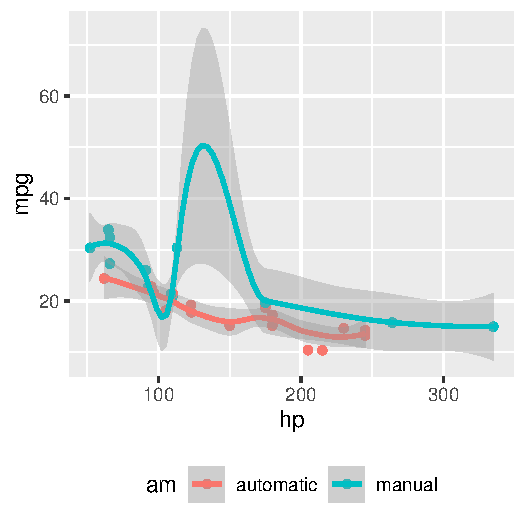
\includegraphics{Shifting_Baselines_files/figure-latex/fig-margin-1} \caption[MPG vs horsepower, colored by transmission]{MPG vs horsepower, colored by transmission.}\label{fig:fig-margin}
\end{marginfigure}

Note the use of the \texttt{fig.cap} chunk option to provide a figure
caption. You can adjust the proportions of figures using the
\texttt{fig.width} and \texttt{fig.height} chunk options. These are
specified in inches, and will be automatically scaled down to fit within
the handout margin.

\hypertarget{arbitrary-margin-content}{%
\subsection{Arbitrary Margin Content}\label{arbitrary-margin-content}}

In fact, you can include anything in the margin using the \textbf{knitr}
engine named \texttt{marginfigure}. Unlike R code chunks
\texttt{\textasciigrave{}\textasciigrave{}\textasciigrave{}\{r\}}, you
write a chunk starting with
\texttt{\textasciigrave{}\textasciigrave{}\textasciigrave{}\{marginfigure\}}
instead, then put the content in the chunk. See an example on the right
about the first fundamental theorem of calculus.

\begin{marginfigure}
We know from \emph{the first fundamental theorem of calculus} that for
\(x\) in \([a, b]\):
\[\frac{d}{dx}\left( \int_{a}^{x} f(u)\,du\right)=f(x).\]
\end{marginfigure}

For the sake of portability between LaTeX and HTML, you should keep the
margin content as simple as possible (syntax-wise) in the
\texttt{marginefigure} blocks. You may use simple Markdown syntax like
\texttt{**bold**} and \texttt{\_italic\_} text, but please refrain from
using footnotes, citations, or block-level elements (e.g.~blockquotes
and lists) there.

Note: if you set \texttt{echo\ =\ FALSE} in your global chunk options,
you will have to add \texttt{echo\ =\ TRUE} to the chunk to display a
margin figure, for example
\texttt{\textasciigrave{}\textasciigrave{}\textasciigrave{}\{marginfigure,\ echo\ =\ TRUE\}}.

\hypertarget{full-width-figures}{%
\subsection{Full Width Figures}\label{full-width-figures}}

You can arrange for figures to span across the entire page by using the
chunk option \texttt{fig.fullwidth\ =\ TRUE}.

\begin{Shaded}
\begin{Highlighting}[]
\FunctionTok{ggplot}\NormalTok{(diamonds, }\FunctionTok{aes}\NormalTok{(carat, price)) }\SpecialCharTok{+} \FunctionTok{geom\_smooth}\NormalTok{() }\SpecialCharTok{+}
  \FunctionTok{facet\_grid}\NormalTok{(}\SpecialCharTok{\textasciitilde{}}\NormalTok{ cut)}
\end{Highlighting}
\end{Shaded}

\begin{figure*}
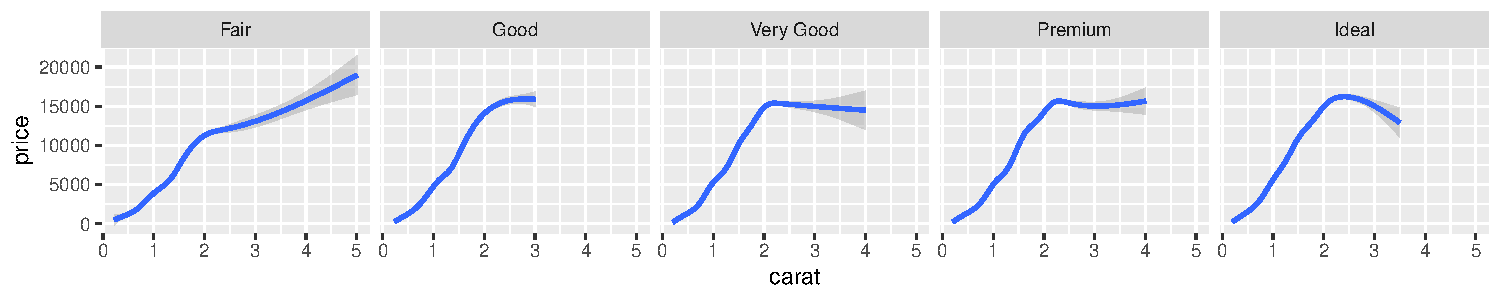
\includegraphics{Shifting_Baselines_files/figure-latex/fig-fullwidth-1} \caption[A full width figure]{A full width figure.}\label{fig:fig-fullwidth}
\end{figure*}

Other chunk options related to figures can still be used, such as
\texttt{fig.width}, \texttt{fig.cap}, \texttt{out.width}, and so on. For
full width figures, usually \texttt{fig.width} is large and
\texttt{fig.height} is small. In the above example, the plot size is
\(10 \times 2\).

\hypertarget{arbitrary-full-width-content}{%
\subsection{Arbitrary Full Width
Content}\label{arbitrary-full-width-content}}

Any content can span to the full width of the page. This feature
requires Pandoc 2.0 or above. All you need is to put your content in a
fenced \texttt{Div} with the class \texttt{fullwidth}, e.g.,

\begin{Shaded}
\begin{Highlighting}[]
\NormalTok{::: \{.fullwidth\}}
\NormalTok{Any \_full width\_ content here.}
\NormalTok{:::}
\end{Highlighting}
\end{Shaded}

Below is an example:

\emph{R is free software and comes with ABSOLUTELY NO WARRANTY.} You are
welcome to redistribute it under the terms of the GNU General Public
License versions 2 or 3. For more information about these matters see
\url{https://www.gnu.org/licenses/}.

\hypertarget{main-column-figures}{%
\subsection{Main Column Figures}\label{main-column-figures}}

Besides margin and full width figures, you can of course also include
figures constrained to the main column. This is the default type of
figures in the LaTeX/HTML output.

\begin{Shaded}
\begin{Highlighting}[]
\FunctionTok{ggplot}\NormalTok{(diamonds, }\FunctionTok{aes}\NormalTok{(cut, price)) }\SpecialCharTok{+} \FunctionTok{geom\_boxplot}\NormalTok{()}
\end{Highlighting}
\end{Shaded}

\begin{figure}
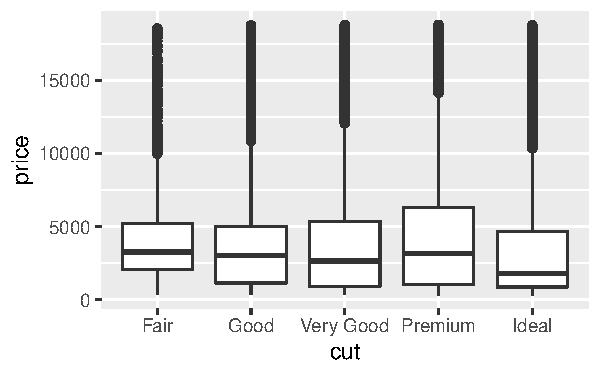
\includegraphics{Shifting_Baselines_files/figure-latex/fig-main-1} \caption[A figure in the main column]{A figure in the main column.}\label{fig:fig-main}
\end{figure}

\hypertarget{sidenotes}{%
\section{Sidenotes}\label{sidenotes}}

One of the most prominent and distinctive features of this style is the
extensive use of sidenotes. There is a wide margin to provide ample room
for sidenotes and small figures. Any use of a footnote will
automatically be converted to a sidenote. \footnote{This is a sidenote
  that was entered using a footnote.}

If you'd like to place ancillary information in the margin without the
sidenote mark (the superscript number), you can use the
\texttt{margin\_note()} function from \textbf{tufte} in an inline R
expression.
\marginnote{This is a margin note.  Notice that there is no number preceding the note.}
This function does not process the text with Pandoc, so Markdown syntax
will not work here. If you need to write anything in Markdown syntax,
please use the \texttt{marginfigure} block described previously.

\hypertarget{references}{%
\section{References}\label{references}}

References can be displayed as margin notes for HTML output. For
example, we can cite R here \citep{R-base}. To enable this feature, you
must set \texttt{link-citations:\ yes} in the YAML metadata, and the
version of Pandoc should at least 2.11 or \texttt{pandoc-citeproc}
should be available and at least 0.7.2. You can always install your own
version of Pandoc from \url{https://pandoc.org/installing.html} if the
version is not sufficient. To check the version of
\texttt{pandoc-citeproc} in your system, you may run this in R:

\begin{Shaded}
\begin{Highlighting}[]
\FunctionTok{system2}\NormalTok{(}\StringTok{\textquotesingle{}pandoc{-}citeproc\textquotesingle{}}\NormalTok{, }\StringTok{\textquotesingle{}{-}{-}version\textquotesingle{}}\NormalTok{)}
\end{Highlighting}
\end{Shaded}

If your version of \texttt{pandoc-citeproc} is too low, or you did not
set \texttt{link-citations:\ yes} in YAML, references in the HTML output
will be placed at the end of the output document.

\hypertarget{tables}{%
\section{Tables}\label{tables}}

You can use the \texttt{kable()} function from the \textbf{knitr}
package to format tables that integrate well with the rest of the Tufte
handout style. The table captions are placed in the margin like figures
in the HTML output.

\begin{Shaded}
\begin{Highlighting}[]
\NormalTok{knitr}\SpecialCharTok{::}\FunctionTok{kable}\NormalTok{(}
\NormalTok{  mtcars[}\DecValTok{1}\SpecialCharTok{:}\DecValTok{6}\NormalTok{, }\DecValTok{1}\SpecialCharTok{:}\DecValTok{6}\NormalTok{], }\AttributeTok{caption =} \StringTok{\textquotesingle{}A subset of mtcars.\textquotesingle{}}
\NormalTok{)}
\end{Highlighting}
\end{Shaded}

\begin{longtable}[]{@{}lrrrrrr@{}}
\caption{A subset of mtcars.}\tabularnewline
\toprule\noalign{}
& mpg & cyl & disp & hp & drat & wt \\
\midrule\noalign{}
\endfirsthead
\toprule\noalign{}
& mpg & cyl & disp & hp & drat & wt \\
\midrule\noalign{}
\endhead
\bottomrule\noalign{}
\endlastfoot
Mazda RX4 & 21.0 & 6 & 160 & 110 & 3.90 & 2.620 \\
Mazda RX4 Wag & 21.0 & 6 & 160 & 110 & 3.90 & 2.875 \\
Datsun 710 & 22.8 & 4 & 108 & 93 & 3.85 & 2.320 \\
Hornet 4 Drive & 21.4 & 6 & 258 & 110 & 3.08 & 3.215 \\
Hornet Sportabout & 18.7 & 8 & 360 & 175 & 3.15 & 3.440 \\
Valiant & 18.1 & 6 & 225 & 105 & 2.76 & 3.460 \\
\end{longtable}

\bibliography{skeleton.bib}



\end{document}
